%%%%%%%%%%%%%%%%%%%%%%%%%%%%%%%%%%%%%%%%%%%%%%
%                insertmeeting
% 1) Title (something creative & funny?)
% 2) Date (MM/DD/YYYY)
% 3) Location (ex. Hagerty High School)
% 4) People/Committees Present 
% 5) Picture 
% 6) Start Time & Stop Time (ex. 12:30AM to 4:30PM)
%%%%%%%%%%%%%%%%%%%%%%%%%%%%%%%%%%%%%%%%%%%%%%
\insertmeeting 
	{Menu Madness!} 
	{02/22/22} 
	{Hagerty High School}
	{James, Jensen, Samantha, Anouska, Annika, Clayton, Falon, Nathan, Ritam}
	{Images/RobotPics/robot.jpg}
	{2:30 - 4:30}
	
\hhscommittee{Software}
\noindent\hfil\rule{\textwidth}{.4pt}\hfil
\subsubsection*{Goals}
\begin{itemize}
    \item Refine menu system for use before autonomous period

\end{itemize} 

\noindent\hfil\rule{\textwidth}{.4pt}\hfil

\subsubsection*{Accomplishments}
The library we use, TRC FTC-lib, there is an option to add options before executing our autonomous program. For us, we wanted to use this to have a master autonomous file that stores all of the programs that we can run. This could improve our debugging abilities and streamline the match process. Currently, we have options to select the alliance, a choice from Near Carousel Warehouse, Near Carousel Storage, and Far Carousel autonomous programs. In addition, we have a final menu if we don't want to park, park in storage, or park in the warehouse. This implementation was relatively simple, and we were able to integrate it into our code without any major obstacles. This will definitely help us at the State championships. 

\begin{figure}[htp]
\centering
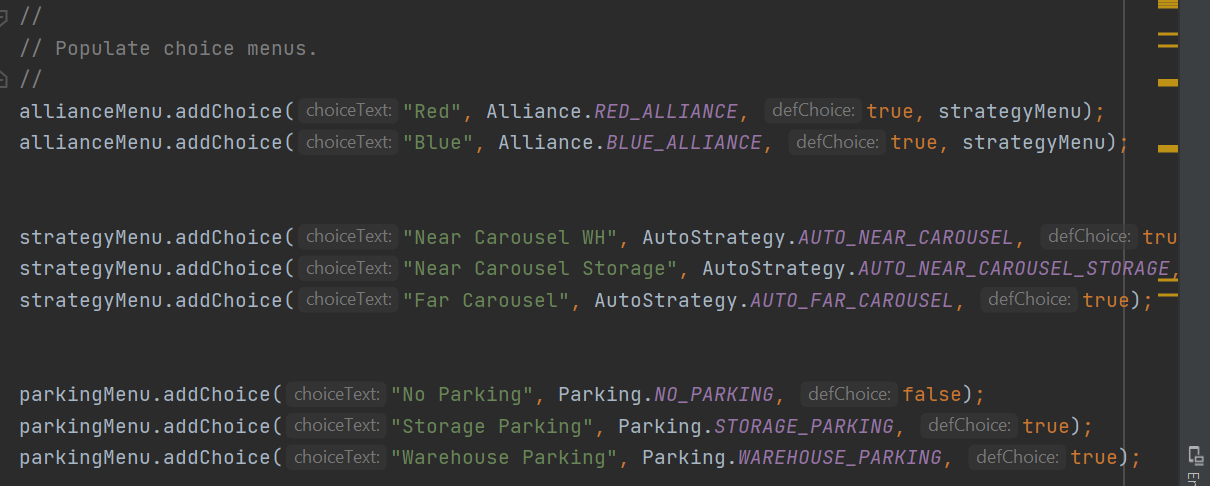
\includegraphics[width=0.95\textwidth, angle=0]{Meetings/February/02-22-22/02-22-22 1.png}
\caption{Our completed code for the autonomous menus.}
\label{fig:022222_1}
\end{figure}


\whatsnext{
\begin{itemize}
    \item Improve the consistency of the autonomous program. 

\end{itemize} 
}

